\chapter{Use with MPLABX}

Use with MPLABX to program and Debug

\section{Installing the Necessary Tools}

\subsection{Install MPLABX IDE and XC8 Compiler}
Links for download  \href{http://www.microchip.com/mplabx}{MPLABX IDE} and \href{http://www.microchip.com/compilers}{XC8 Compiler} installers.
Download and install.

\subsection{Install PICsimLab}

Link for download \href{http://sourceforge.net/projects/picsim/files/picsim/picsim-0.6/}{PICsimLab-0.6} installer. 
Download and install

\subsection{How to Install PicsimLab MPLABX Debugger plugin}

Link for download \href{http://sourceforge.net/projects/picsim/files/picsim/picsim-0.6/}{PicsimLab MPLABX Debugger plugin (com-picsim-picsimlab.nbm)} 

\begin{figure}[H]
\center
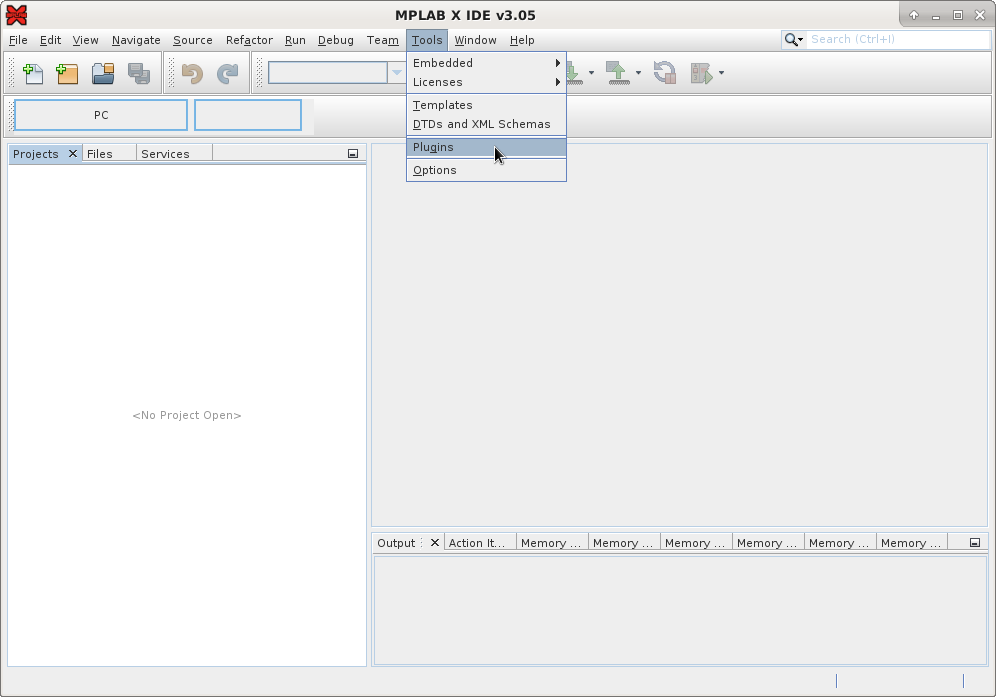
\includegraphics[width=0.98\textwidth]{img/hmd/mplab01.png} 
\end{figure} 

\begin{figure}[H]
\center
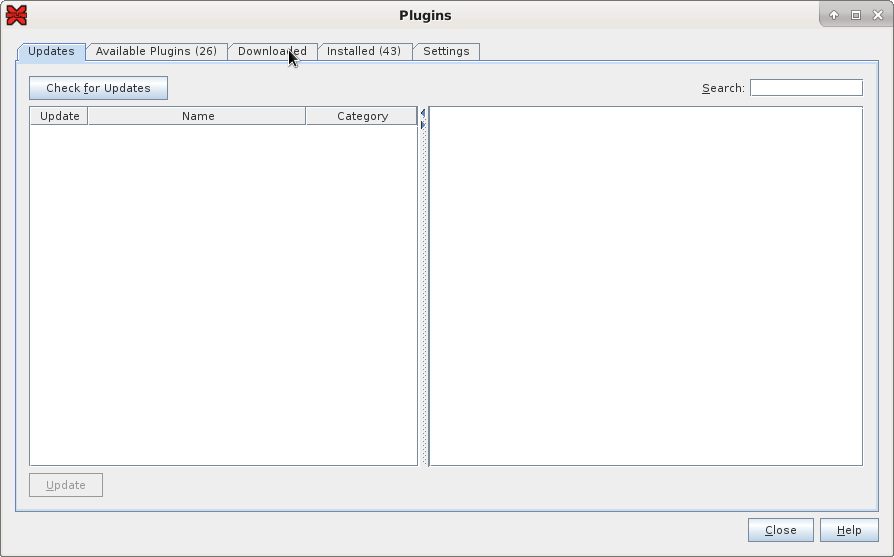
\includegraphics[width=0.8\textwidth]{img/hmd/mplab02.png} 
\end{figure} 

\begin{figure}[H]
\center
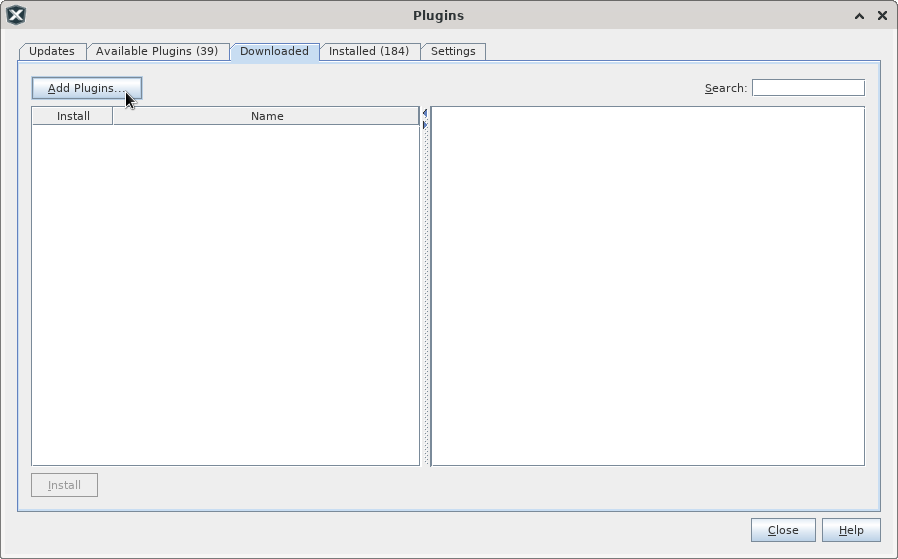
\includegraphics[width=0.98\textwidth]{img/hmd/mplab03.png} 
\end{figure} 

\begin{figure}[H]
\center
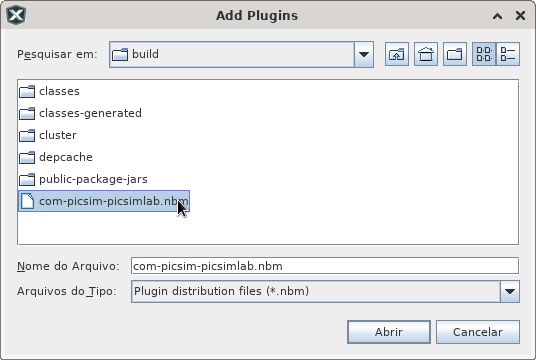
\includegraphics[width=0.6\textwidth]{img/hmd/mplab04.png} 
\end{figure} 

\begin{figure}[H]
\center
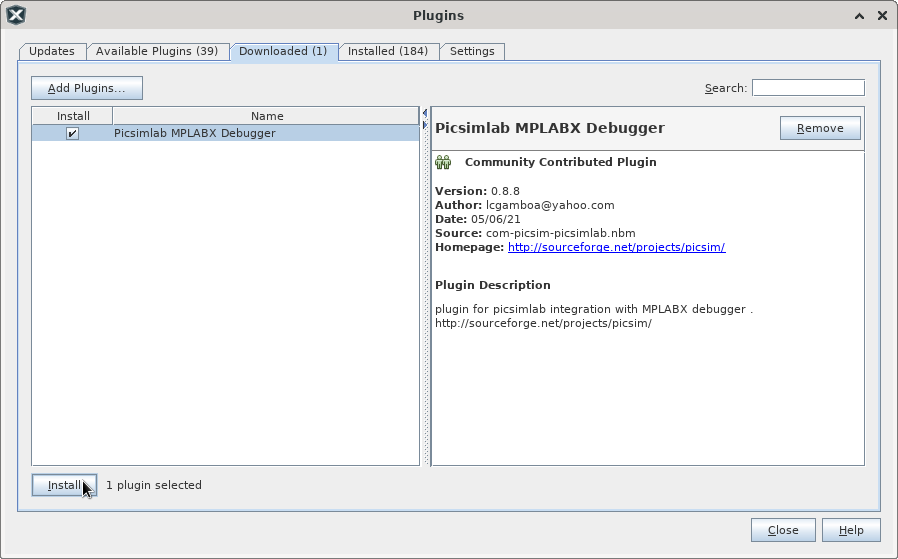
\includegraphics[width=0.98\textwidth]{img/hmd/mplab05.png} 
\end{figure} 


\begin{figure}[H]
\center
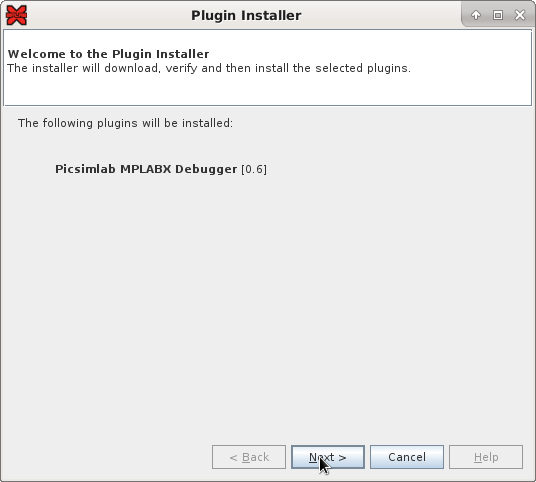
\includegraphics[width=0.7\textwidth]{img/hmd/mplab06.png} 
\end{figure} 

\begin{figure}[H]
\center
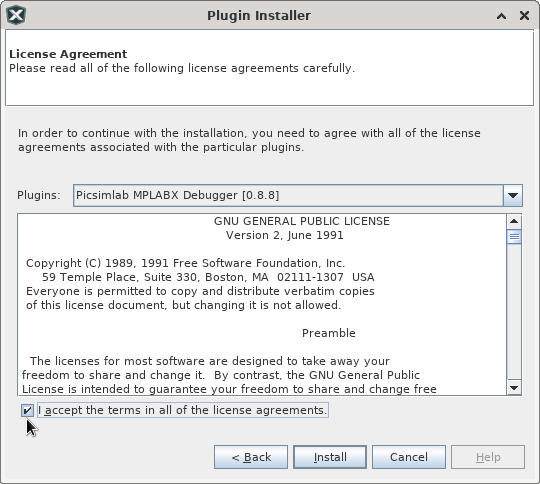
\includegraphics[width=0.7\textwidth]{img/hmd/mplab07.png} 
\end{figure} 

\begin{figure}[H]
\center
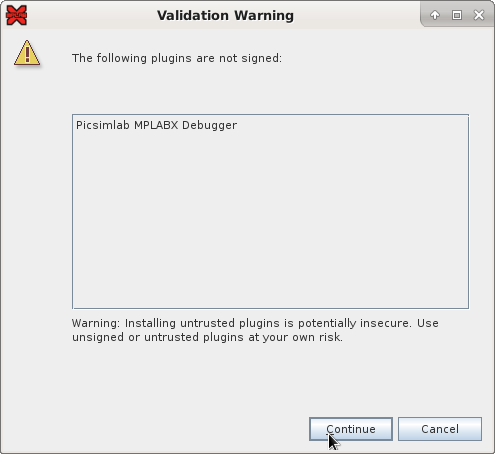
\includegraphics[width=0.7\textwidth]{img/hmd/mplab08.png} 
\end{figure} 

\begin{figure}[H]
\center
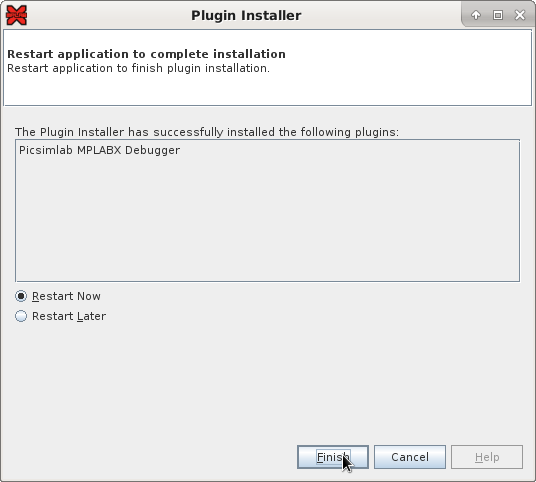
\includegraphics[width=0.7\textwidth]{img/hmd/mplab09.png} 
\end{figure} 


\section{Configuring a New Project in MPLABX}

\subsection{Project Creation}

\begin{figure}[H]
\center
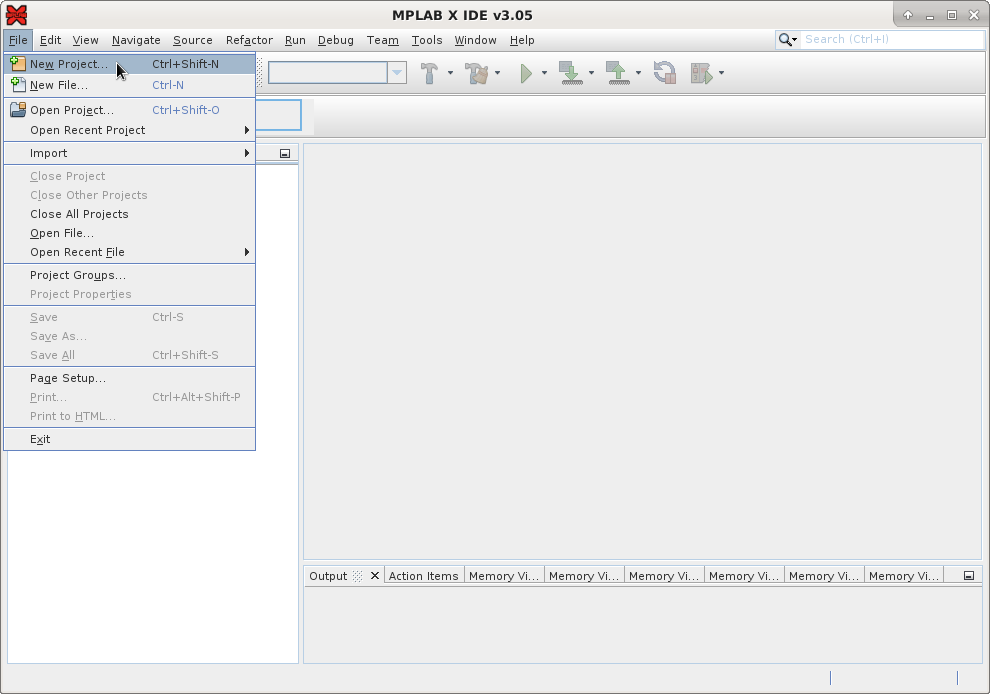
\includegraphics[width=0.98\textwidth]{img/hmd/mplab10.png} 
\end{figure} 

\begin{figure}[H]
\center
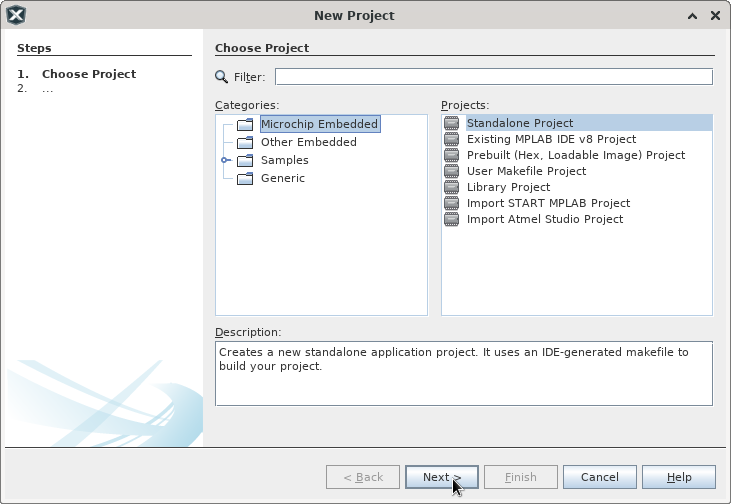
\includegraphics[width=0.71\textwidth]{img/hmd/mplab11.png} 
\end{figure} 

\begin{figure}[H]
\center
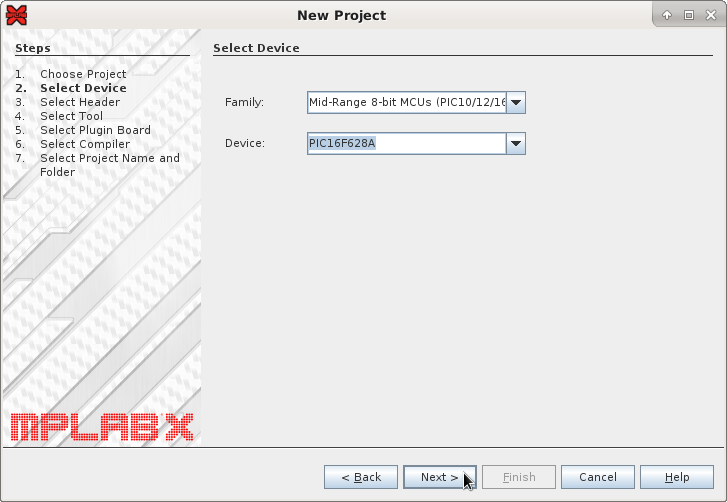
\includegraphics[width=0.71\textwidth]{img/hmd/mplab12.png} 
\end{figure}

\begin{figure}[H]
\center
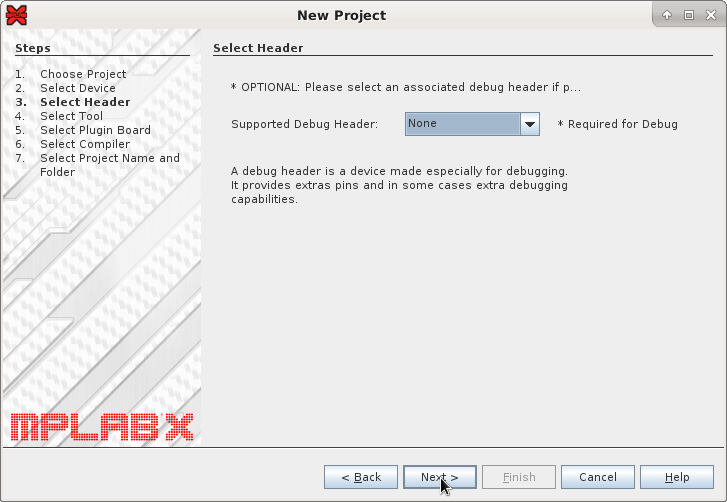
\includegraphics[width=0.71\textwidth]{img/hmd/mplab13.png} 
\end{figure} 

\begin{figure}[H]
\center
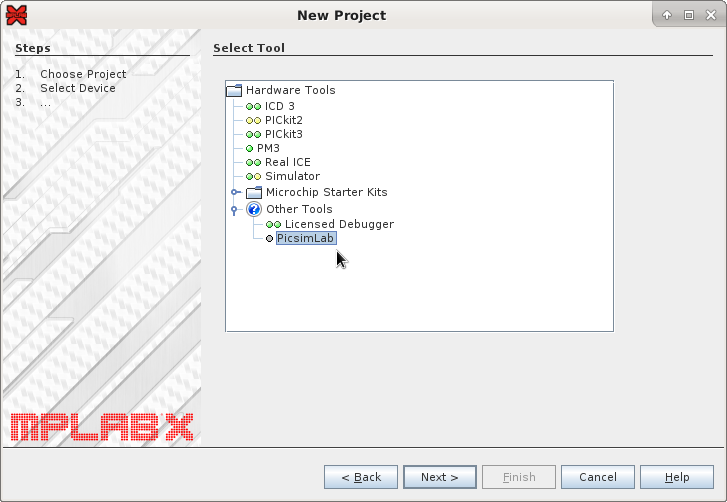
\includegraphics[width=0.71\textwidth]{img/hmd/mplab14.png} 
\end{figure} 

\begin{figure}[H]
\center
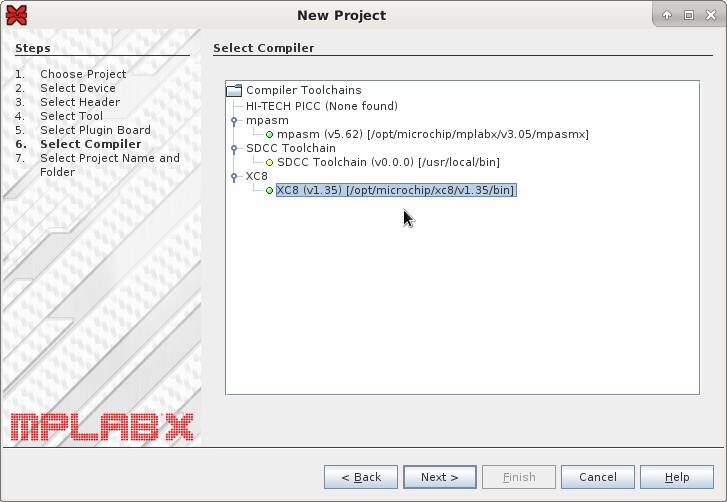
\includegraphics[width=0.71\textwidth]{img/hmd/mplab15.png} 
\end{figure} 

\begin{figure}[H]
\center
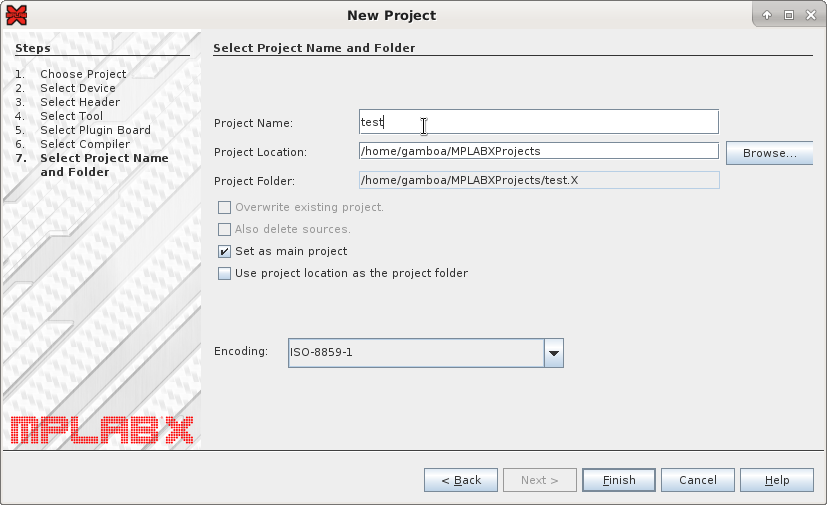
\includegraphics[width=0.71\textwidth]{img/hmd/mplab16.png} 
\end{figure} 

\subsection{File Creation}

\begin{figure}[H]
\center
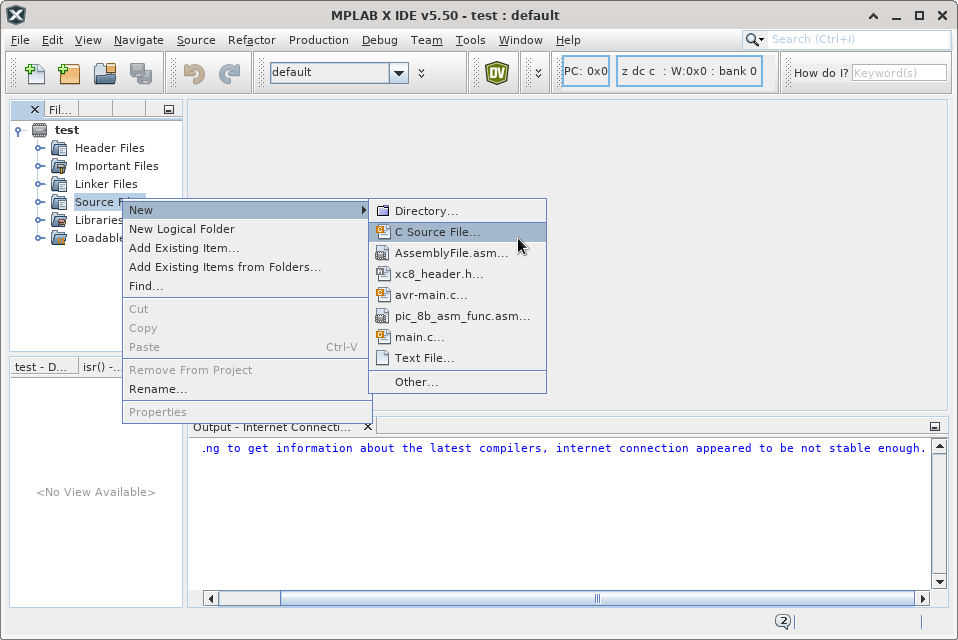
\includegraphics[width=0.98\textwidth]{img/hmd/mplab17.png} 
\end{figure} 

\begin{figure}[H]
\center
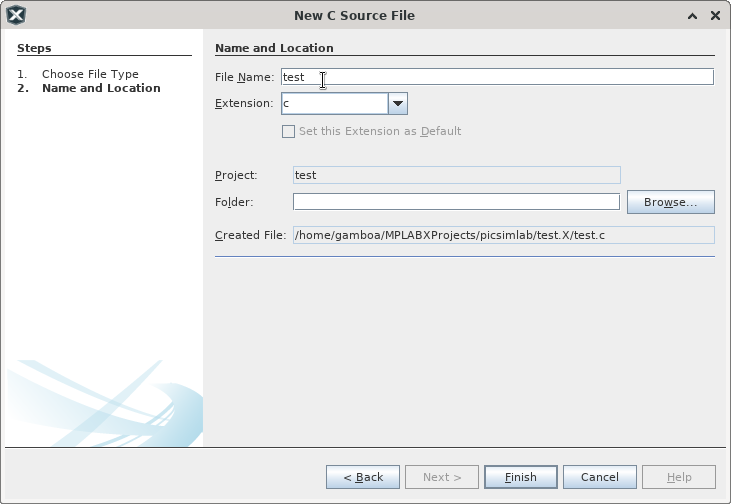
\includegraphics[width=0.8\textwidth]{img/hmd/mplab18.png} 
\end{figure} 


\subsection{PIC Configuration Bits}
\begin{figure}[H]
\center
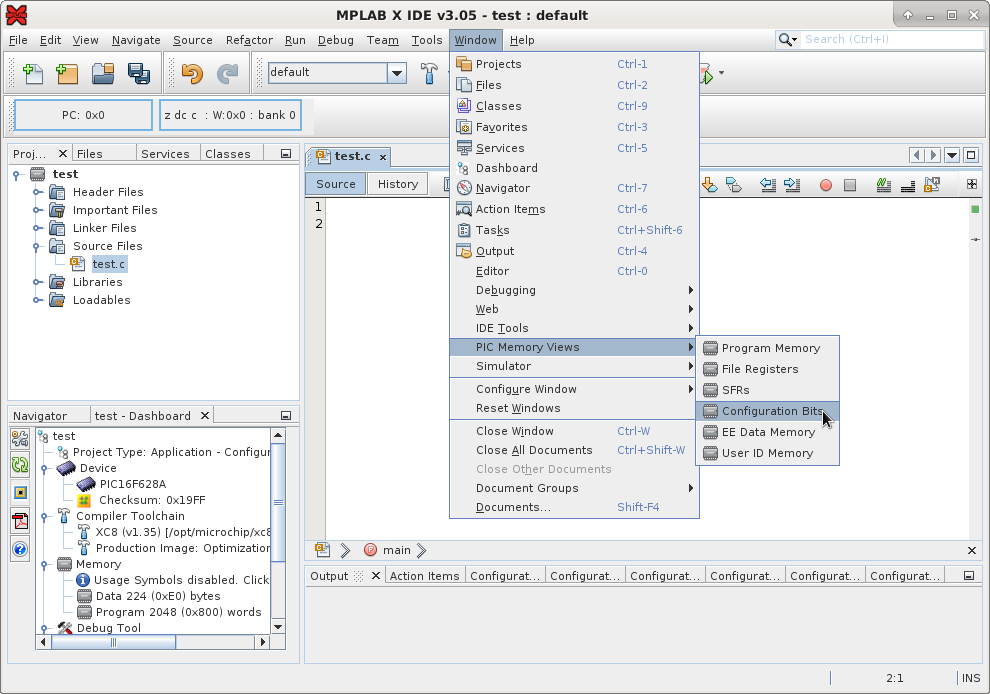
\includegraphics[width=0.98\textwidth]{img/hmd/mplab19.png} 
\end{figure} 

\begin{figure}[H]
\center
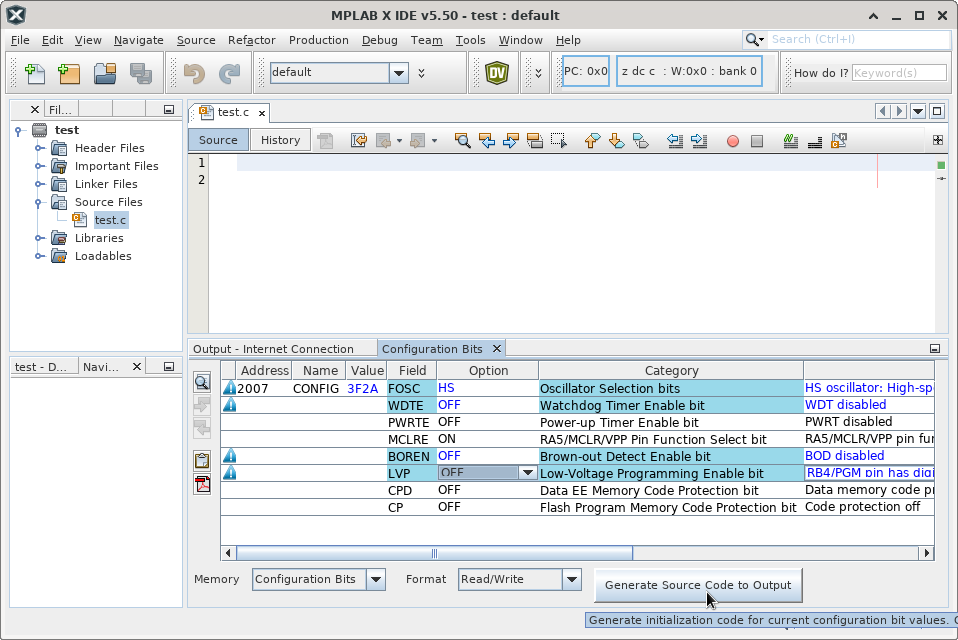
\includegraphics[width=0.98\textwidth]{img/hmd/mplab20.png} 
\end{figure} 


\begin{figure}[H]
\center
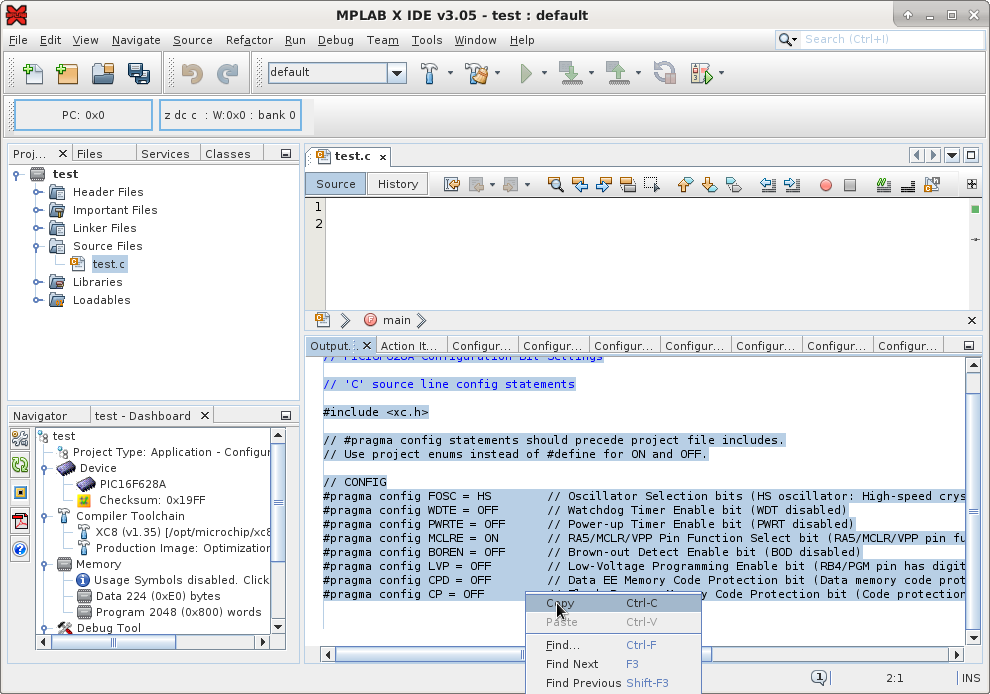
\includegraphics[width=0.98\textwidth]{img/hmd/mplab21.png} 
\end{figure} 

\subsection{Code Example}

Paste the configuration and this simple code example in test.c:
\begin{minted}{c}
void main()
{
    TRISB=0x00; //All pins as output
    PORTB=0;    //All pins off
    while(1)    //main loop
    {
        PORTBbits.RB0=1; //Turn RB0 on
        PORTBbits.RB1=1; //Turn RB1 on
        PORTB=0;  //All pins off
    }
}
\end{minted}


\begin{figure}[H]
\center
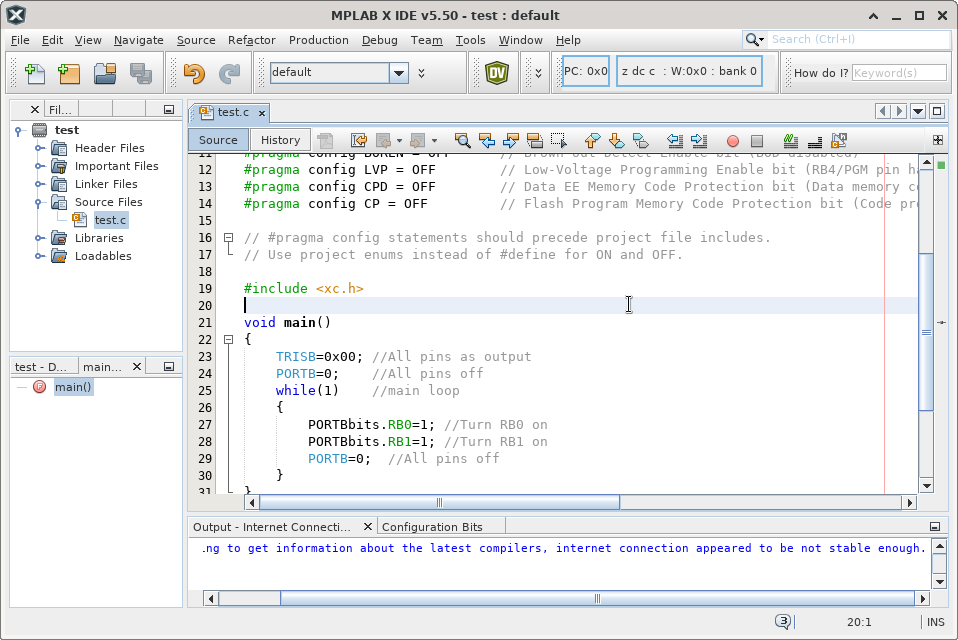
\includegraphics[width=0.98\textwidth]{img/hmd/mplab22.png} 
\end{figure} 

\subsection{Building the Project}

Use the \textbf{Build} button and wait for the message ``\textcolor{green}{BUILD SUCCESSFUL}''.

\begin{figure}[H]
\center
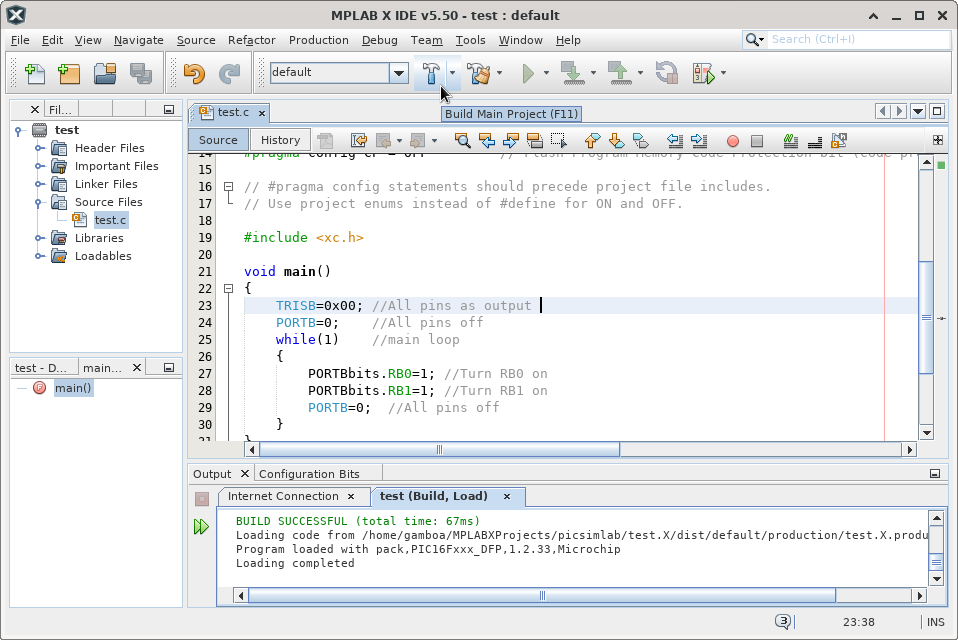
\includegraphics[width=0.98\textwidth]{img/hmd/mplab23.png} 
\end{figure} 



\section{Program and Debug PICsimLab With MPLABX}


\subsection{Starting PICsimLab}
\begin{figure}[H]
\center
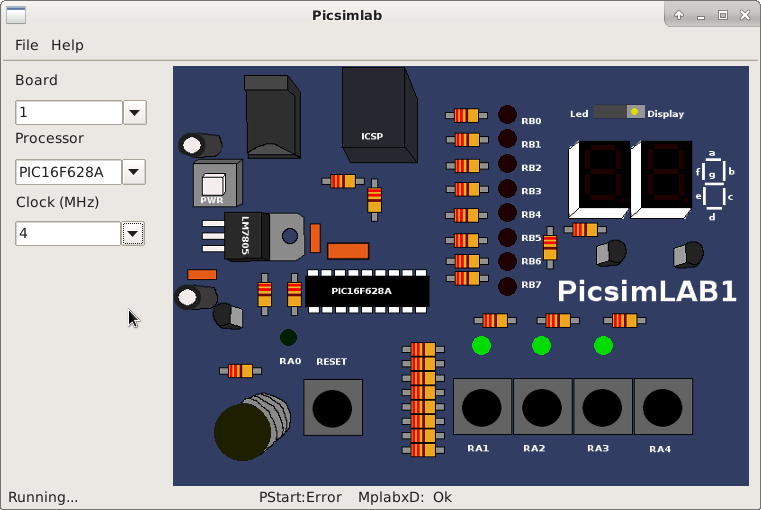
\includegraphics[width=0.8\textwidth]{img/hmd/mplab24.png} 
\end{figure} 

The plugin connect to Picsimlab through a TCP socket using port 1234, and you have to allow the access in the firewall. Verify in the PICsimLab statusbar the message ``MplabxD: Ok''. It's show debugger server state.


\subsection{Programming PICsimLab}

Use the \textbf{Debug} button to programming PICsimLab.  
\begin{figure}[H]
\center
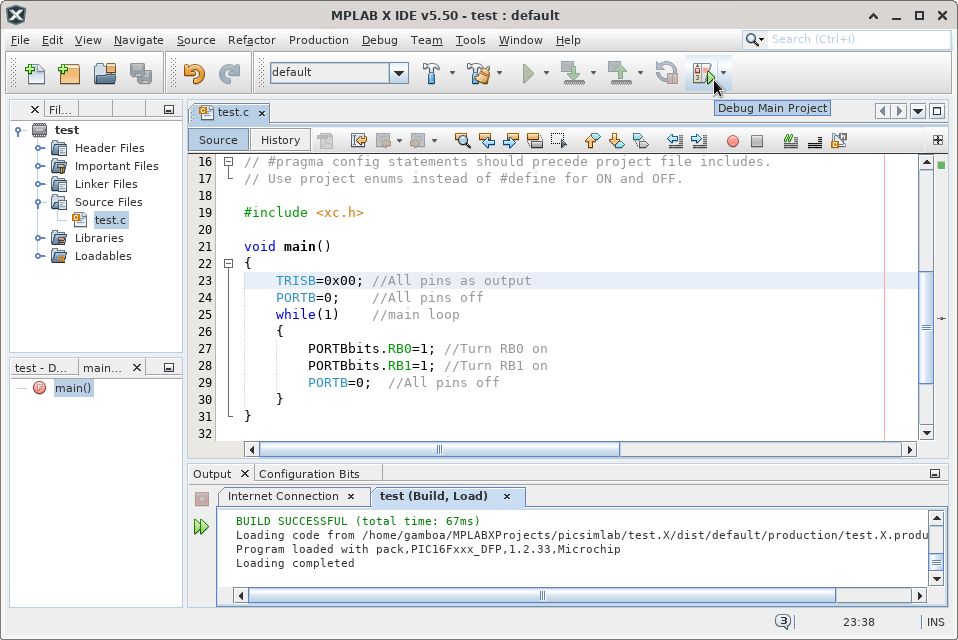
\includegraphics[width=0.98\textwidth]{img/hmd/mplab25.png} 
\end{figure} 

\subsection{Pausing the Program}
Use the \textbf{Pause} button to stop the program and inspect the code and memory.
\begin{figure}[H]
\center
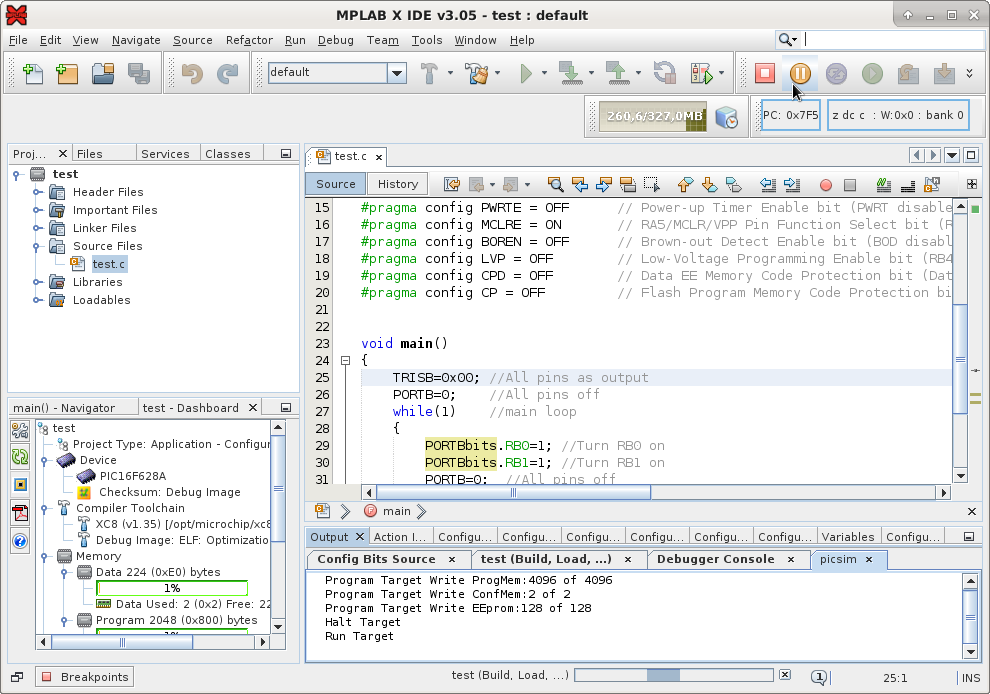
\includegraphics[width=0.98\textwidth]{img/hmd/mplab26.png} 
\end{figure} 

\subsection{Restarting the Program}
Use the \textbf{Restart} button to restart the program.
\begin{figure}[H]
\center
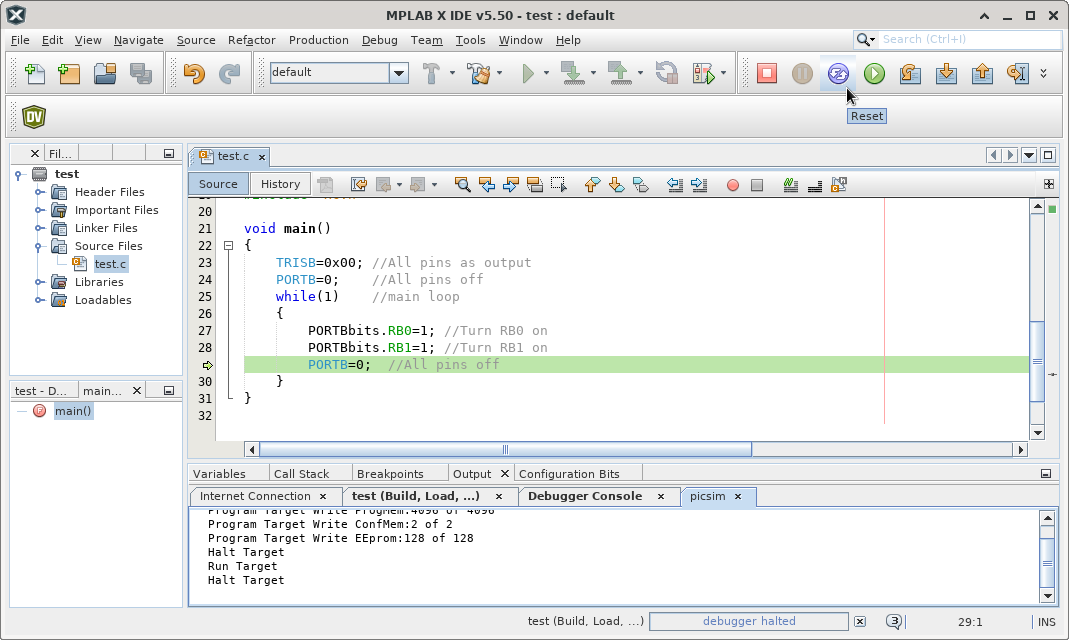
\includegraphics[width=0.98\textwidth]{img/hmd/mplab27.png} 
\end{figure} 

\subsection{Running Step by Step}
Use the \textbf{Step} or \textbf{Step Over} button to run the program step by step.
\begin{figure}[H]
\center
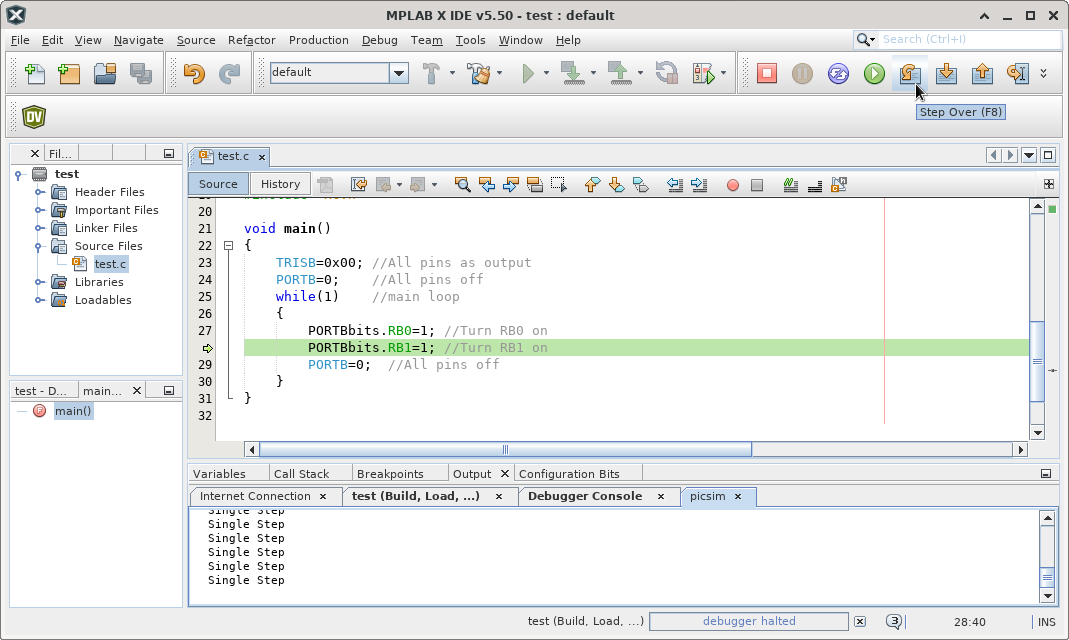
\includegraphics[width=0.98\textwidth]{img/hmd/mplab28.png} 
\end{figure} 

See in the PICsimLab the changes of each step.
\begin{figure}[H]
\center
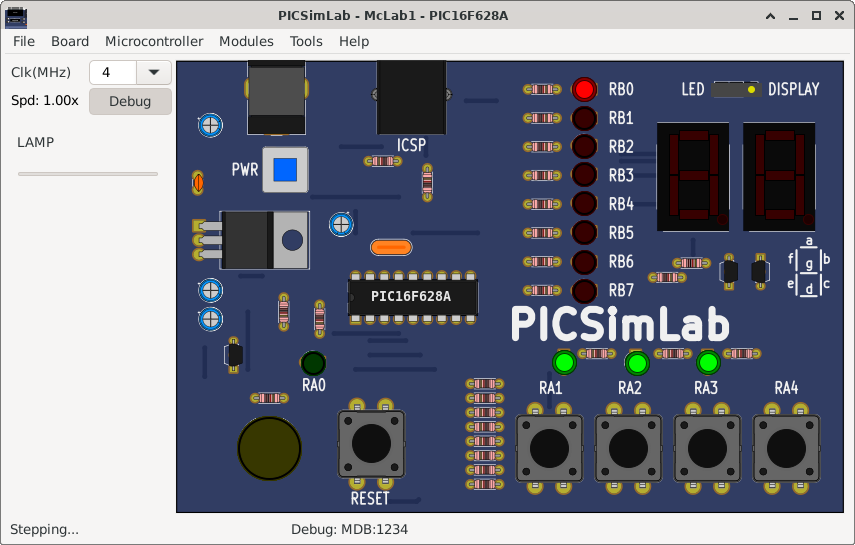
\includegraphics[width=0.8\textwidth]{img/hmd/mplab29.png} 
\end{figure} 

\subsection{Stopping Debugger}
Use the \textbf{Stop} button to turn off the MPLABX debugger. The program continues running in PICsimLab after MPLABX debugger is stopped.
\begin{figure}[H]
\center
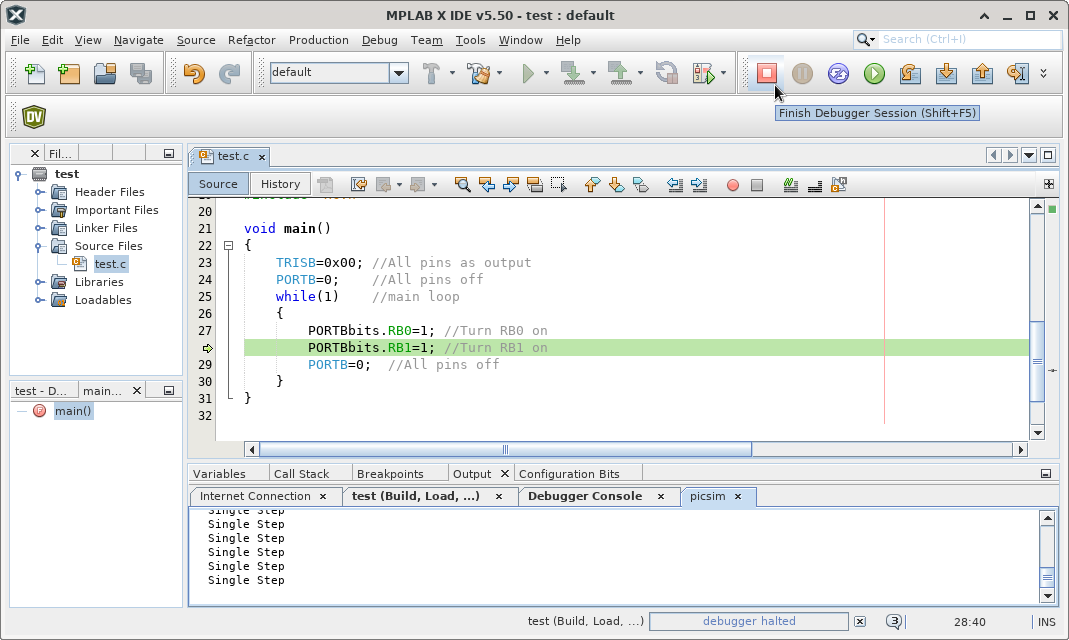
\includegraphics[width=0.98\textwidth]{img/hmd/mplab30.png} 
\end{figure} 


\section{This Tutorial in Video}

Link for Youtube video version of this tutorial: \href{https://youtu.be/q2oZB50Avm4}{How to use MPLABX to program and debug PicsimLab 0.6}


